\chapter{Induced interaction, effective Hamiltonian and topology} % Main chapter title

\label{Chapter7} 

\lhead{Part IV. \emph{Kitaev chain}}
\chead{Chapter 7. \emph{Interaction, Hamiltonian \& topology}} % This is for the header on each page - perhaps a shortened title
%----------------------------------------------------------------------------------------
In this chapter we derive the effective Hamiltonian for the fermionic chain. We start off by going back to the Bose gas and consider the effect of making the gas one-dimensional. See section \ref{sec.1DBosegas}. In section \ref{sec.TightbindingHam.lattice} we introduce the tight-binding Hamiltonian for the lattice fermions. In section \ref{sec.interaction.lattice} we calculate the induced interaction and write up the effective interaction Hamiltonian for the fermions. In section \ref{sec.grandhamiltonian.lattice} we outline the mean field approximation and write doen the effective BCS Hamiltonian. Finally, in section \ref{sec.topology.lattice} we discuss the topology of the system and calculate the topological index.

\section{1D Bose gas} \label{sec.1DBosegas}
In this section we will use Bogoliubov theory to describe the uniform one-dimensional Bose gas. The uniform Bose gas does not show true Bose-Einstein condensation in one dimension. However, in two historical papers by Lieb and Liniger exact solutions for the one-dimensional Bose gas are studied. They find, that the Bogoliubov theory gives the correct excitation spectrum for a weakly interacting gas \cite{LiebLiniger1, LiebLiniger2}. Further from a more recent paper it is evident, that for weak interactions the density-density correlation function is also well-described within Bogoliubov theory \cite{Calabrese}. Since it is exactly the density-density correlation function, that is important for our studies, it is justifiable to use Bogoliubov theory.

Going back to equation \eqref{eq.BECHamiltonianrealspace} we have the real space expansion of the Hamiltonian for the bosons:
\begin{equation}
H_{BB} = \int d^3 r \left(\psi_B^\dagger(\mathbf{r})\left[-\frac{\nabla^2}{2m_B}\right]\psi_B(\mathbf{r}) + \frac{g_B}{2}\psi_B^\dagger(\mathbf{r})\psi_B^\dagger(\mathbf{r})\psi_B(\mathbf{r})\psi_B(\mathbf{r})  \right), \nonumber
\end{equation}
We assume, that the bosons are trapped along the $x$-axis and that the energy required to be excited in the transverse direction is much larger than the typical energy of the bosons. This means, that we can make the following expansion for the bosons:
\begin{equation}
\psi_B(x, \mathbf{r}_{\perp}) = \phi_0(\mathbf{r}_{\perp}) \psi_B(x) = \frac{1}{\sqrt{\mathcal{L}}} \sum_k \text{e}^{ikx} \phi_0(\mathbf{r}_{\perp}) b_k, 
\nonumber
\end{equation}
where $\phi_0(\mathbf{r}_\perp) = \frac{1}{\sqrt{\pi}l_t}\text{e}^{-r_{\perp}^2/2l_t^2}$ is the harmonic ground state of the transverse directions with trapping width $l_t$. Inserting this expansion into the quartic interaction part of the Hamiltonian yields:
\begin{equation}
H_{BB}^{\text{int}} = \frac{g_B}{2}\int d^3 r \; \psi_B^\dagger(\mathbf{r})\psi_B^\dagger(\mathbf{r})\psi_B(\mathbf{r})\psi_B(\mathbf{r}) = \frac{g_B}{2\pi l_t^2}\frac{1}{2\mathcal{L}}\sum_{k_1,k_2,q} b^\dagger_{k_1 + q}b^\dagger_{k_2 - q}b_{k_1}b_{k_2}. \nonumber
\end{equation}
We see, that this has the exact same form as the momentum space interaction Hamiltonian for the 3D gas contained in equation \eqref{eq.BECHamiltonianmomentumspace}. Further they are equivalent under the identification $g_B \to \frac{g_B}{2\pi l_t^2}$. We could now carry through the condensate approximation with $\psi_B(x) = \sqrt{n_B} + \delta\psi_B(x)$ with the last term being small and containing the $k \neq 0$ terms, and $n_B = \frac{N_B}{\mathcal{L}}$. The numerics are exactly the same as before, under the above change of $g_B$ and $n_B$. Hence, in this approximation we get the same properties of the one-dimensional gas. The Green's functions of section \ref{sec.BECGreens} is altered only in the change of $g_B$ and $n_B$. The Bose gas parameter is now $n_Ba_B$ and in turn the coherence length is: $\xi = \frac{l_t}{2\sqrt{n_Ba_B}}$. We are thus ready to calculate the induced interaction for the fermions once again. 

In appendix \ref{Appendix.groundstatedepletion.1DBosegas} we have calculated the ground state depletion of the Bose gas. For Bogoliubov theory to be self-consistent this depletion must be small. From equation \eqref{eq.groundstatedepletion.1Dbosegas} we get, that in the thermodynamic limit the depletion diverges $\propto \ln\left(\frac{\sqrt{2}\mathcal{L}}{\pi\xi} \right)$. This emphasizes, that the Bogoliubov theory is only applicable for a \textit{finite} system in this one-dimensional case and once again illuminates the difficulties of using mean field theory in one dimension, as discussed in section \ref{sec.meanfieldvalidity}. For a finite system the depletion can be controlled to be small by increasing the boson density, $n_B$. 

\section{Tight-binding Hamiltonian} \label{sec.TightbindingHam.lattice}
To get familiar with the relevant energy and length scale we now turn to the tight-binding Hamiltonian.

The fermions are arranged in a one dimensional optical lattice with lattice constant $d$ and $N$ sites. The Hamiltonian for nearest and next-nearest hopping is then:
\begin{equation}
H_{0} = \frac{1}{2}\sum_{j} \left[- t_1(c^\dagger_{j+1}c_j + c^\dagger_j c_{j + 1}) - t_2(c^\dagger_{j + 2}c_j + c^\dagger_j c_{j + 2}) \right].
\label{eq.Htightbindingrealspace} 
\end{equation}
Here $c_j$ is a fermionic annihilation operator for a fermion in site $j$. $t_1$ and $t_2$ are the energies associated with nearest neighbour and next-nearest neighbour hopping respectively. In a statical lattice the next-nearest neighbour hopping is ordinarily several orders of magnitude smaller than $t_1$. However, by shaking the optical lattice one can effectively tune the next-nearest hopping to be large. Hence, it is possible to investigate the entire range of: $t_2 / t_1 \in (0, \infty)$ \cite{Liberto.ShakingOpticalLattice}. 

We define the momentum space operators through: $c_j = \frac{1}{\sqrt{N}}\sum_{k} c_k \text{e}^{ikx_j}$, where $kd = \frac{2\pi n}{N}$ are the allowed momenta for $n = -\frac{N}{2}, \dots, \frac{N}{2} - 1$ for periodic boundary conditions and $x_j = jd$ the positions of the fermions. Inserting this into the above transforms the Hamiltonian to momentum space:
\begin{equation}
H_{0} = \sum_k \left[ - t_1\cos(kd) - t_2\cos(2kd)\right]c^\dagger_kc_k.
\label{eq.Htightbindingmomentumspace} 
\end{equation}
In this sense, we can already see, that going from the gas to the chain corresponds to letting $\frac{k^2}{2m_F} \to - t_1\cos(kd) - t_2\cos(2kd)$. We therefore use $d$ as the unit of length and $t_1$ as the unit of energy. 


\section{Interaction Hamiltonian} \label{sec.interaction.lattice}
We return to the Bose-Fermi interaction Hamiltonian of equation \eqref{eq.HintBF}:
\begin{equation}
H_{BF}^\text{int} = g_{BF}\int d^3 r \; \psi_F^\dagger(\mathbf{r}) \psi_B^\dagger(\mathbf{r})\psi_B(\mathbf{r})\psi_F(\mathbf{r}),
\end{equation} 
This time around we trap the fermions along a wire as before \textit{and} in a lattice. Assuming, that the trapping frequency, $\omega_t$ for the perpendicular directions to the wire is large with respect to the typical energy $t_1$ means, that the fermions are trapped in the harmonic oscillator ground state like the bosons, i.e. the gaussian: $\phi_0(\mathbf{r}_{\perp})$ of width $l_t = \frac{1}{\sqrt{m_F\omega_t}}$. Further, the lattice confinement means, that the states can be expanded in terms of well-localised (orthonormal) Wannier states around the lattice points $x_j = jd$, $d$ being the lattice constant. We approximate these states with gaussians $\phi_0(x - x_j)$ of width $l_x$. In this sense, we expand the field operators according to:
\begin{equation}
\psi_F(x, \mathbf{r}_{\perp}) = \sum_j \phi_0(\mathbf{r}_{\perp})\phi_0(x - x_j) c_j, 
\end{equation}
where $c_j$ annihilates a fermion at site $j$. Inserting this into the interaction Hamiltonian along with the expansion for the bosons, we get:
\begin{equation}
H_{BF}^{\text{int}} = \frac{g_{BF}}{2\pi l_t^2}\frac{1}{\mathcal{L}}\sum_{p_1, p_2, q} c^\dagger_{p_1 - q}b^\dagger_{p_2 + q}b_{p_2}c_{p_1}. \nonumber
\end{equation}
Here we have taken the $l_x \to 0$ limit and used that $c_j = \frac{1}{\sqrt{N}}\sum_p \text{e}^{ipx_j}c_p$. This is equivalent to the Kitaev wires in the 3D Bose gas by letting $g_{BF} \to \frac{g_{BF}}{2\pi l_t^2}$. The calculation of the induced interaction is therefore only altered in the sense, that we should not integrate over the perpendicular directions. This is because, the bosons are now also confined to move in one direction. See section \ref{sec.1D3Dinducedinteraction} for the details. Hence, the Fourier transform of the real space interaction is simply given by equation \eqref{eq.V11indXBEC} without the double integration and by letting $g_B \to \frac{g_B}{2\pi l_t^2}, g_{BF} \to \frac{g_{BF}}{2\pi l_t^2}$ and $n_B = \frac{N_B}{\mathcal{L}}$:
\begin{equation}
V_{\text{ind}}(q, i\omega_q) = \left(\frac{g_{BF}}{2\pi l_t^2}\right)^2 \chi_\text{BEC}(q, i\omega_q), 
\label{eq.VFFmomentumspace.kitaevchain}
\end{equation}
with $\chi_\text{BEC}(q, i\omega_q) = \frac{q^2}{m_B}\frac{n_B}{(i\omega_q)^2 - E_{B,q}^2}$ the density-density correlation function of the BEC. The change of $g_B$ means, that the Bogoliubov spectrum $E_{B,q}$ is altered to: $E_{B,q}^2 = \frac{q^2}{2m_B}\left(\frac{q^2}{2m_B} + 2n_B\frac{g_B}{2\pi l_t^2}\right)$.\footnote{Since the coherence length is similarly altered, the spectrum expressed in terms of the coherence length is unaltered.} The real space interaction is obtained by a Fourier transformation of the above. As for the double wire system we focus on the $\omega_q = 0$ component, whereby we do not take retardation effects into account. However, we wish to consider long coherence lengths, so it is worth discussing these effects. An upper bound for the momentum is provided by the Brillouin zone: $k_F \approx \frac{\pi}{d}$. This means, that the relevant speed of the fermions is $v_F = \frac{k_F}{m_F} = \frac{\pi}{m_Fd}$. Letting $g_B \to \frac{g_B}{2\pi l_t^2}$ means, that the speed of the bosonic Bogoliubov excitations is: $c_0 = \frac{1}{\sqrt{2}m_B\xi}$. The ratio of the velocities hereby becomes: $\frac{v_F}{c_0} = \sqrt{2}\pi\frac{m_B}{m_F}\frac{\xi}{d}$. The retardation effects are only negligible when $v_F\ll c_0$. This means, that either the mass ratio must be unrealistically small, or $\xi \approx d$. Since we wish to consider coherence lengths that are several times the lattice spacing, retardation effects \textit{will} be quantitatively significant. However, we speculate that the zero frequency component will give us qualitatively correct results. The zero frequency component of the real space interaction is:
\begin{equation}
\tilde{V}_{\text{ind}}(x, 0) = \int \frac{dq}{2\pi} \; \text{e}^{iqx}V_{\text{ind}}(q, 0) = -\frac{n_Bg_{BF}^2m_B}{\pi^2l_t^4}\int \frac{dq}{2\pi} \; \text{e}^{iqx} \frac{1}{q^2 + 2/\xi^2}. \nonumber
\end{equation}
This integration can be performed using Cauchy's residue theorem. The result is:
\begin{equation}
\tilde{V}_{\text{ind}}(j, l, 0) = -\frac{n_Bg_{BF}^2m_B}{2\sqrt{2}\pi^2l_t^4}\xi \cdot \text{e}^{-\frac{\sqrt{2}|x_j - x_l|}{\xi}},
\label{eq.Inducedcinteractionrealspace.kitaevchain}
\end{equation}
where we have put $x = x_j - x_l$, the distance between sites $j$ and $l$. From this it is clear what the effect is of making the boson gas one-dimensional. The induced interaction is no longer of the Yukawa form, it is purely exponential. This also means, that we can effectively make the interaction over a range of the lattice constant by making the coherence length large enough. The unitless form of this interaction is obtained by dividing by the nearest neighbour hopping $t_1$:
\begin{equation}
\frac{\tilde{V}_{\text{ind}}(j, l, 0)}{t_1} = -G \cdot \text{e}^{-\frac{\sqrt{2}|x_j - x_l|}{\xi}}, \hspace{0.5cm} G = \frac{\sqrt{2}}{\pi^2} \left(\frac{m_F}{m_B} + \frac{m_B}{m_F} + 2\right)\frac{\varepsilon_0}{t_1}\left(\frac{d}{l_t}\right)^3 \frac{(n_Ba_{BF})^2}{n_Bd\sqrt{n_Ba_B}},
\label{eq.Inducedcinteractionrealspaceunitless.kitaevchain} 
\end{equation}
where $G$ is a measure of the strength of the interaction. Here $\varepsilon_0 = \frac{\pi^2}{2m_Fd^2}$ is the energy of a single fermion in an infinite square well of width $d$. We hereby choose to express the system using the independent variables: $\frac{m_B}{m_F}, n_Bd, \frac{\varepsilon_0}{t_1}, n_B a_{BF}$, and finally the Bose gas parameter: $n_B a_{B}$. In this we assume, that we can separately control the hoppings $t_1, t_2$ and the lattice constant $d$. This is the reason for the additional parameter $\frac{\varepsilon_0}{t_1}$. Instead of specifying this large amount of parameters, we will simply set an overall interaction strength $G$ and use the Bose gas parameter, $n_B a_{B}$, to control the coherence length, $\xi$. Dropping the $0$ in the induced interaction, we can hereby write the fermion interaction Hamiltonian in the zero frequency limit as:
\begin{equation}
H^{\text{int}}_{FF} = \frac{1}{2}\sum_{j,l} c^\dagger_j c^\dagger_l \tilde{V}_{\text{ind}}(j, l) c_l c_j
\label{eq.Hintrealspace.lattice}
\end{equation}
Using the Fourier decomposition $c_j = \frac{1}{\sqrt{N}}\sum_k \text{e}^{ikx_j}c_k$, we transform this to momentum space:
\begin{align}
H^{\text{int}}_{FF} &= \frac{1}{2N} \sum_{k, q, p} W_{\text{ind}}(k, q, p) c^\dagger_{k + p} c^\dagger_{q - p} c_q c_k, \nonumber \\  
W_{\text{ind}}(k, q, p) &= \frac{1}{2}\sum_{j\neq 0} \left[\cos(px_j) - \cos((k - q + p)x_j) \right]\tilde{V}_{\text{ind}}(0, j). 
\label{eq.Hintmomentumspace.lattice}
\end{align}
We notice, that $W_{\text{ind}}(k, q, p)$ is explicitly periodic in the Brillouin zone of width $2\pi / d$. The functional difference between the wire and the lattice is, that the momentum space interaction $W_{\text{ind}}(k, q, p)$ is a finite sum of components of the real space interaction $\tilde{V}_{\text{ind}}(0, j)$, not a combination of Fourier transforms.

\section{Effective Hamiltonian, gap equation and filling fraction} \label{sec.grandhamiltonian.lattice}
The BCS mean field approximation is performed in exactly the same way as for the Kitaev wires. The sum in equation \eqref{eq.Hintmomentumspace.lattice} is truncated to $q = -k$, and the operator $c_kc_{-k}$ is written as it's mean plus a deviation. The deviation is then only kept up to first order. See section \ref{sec.meanfieldapproximation} for the details. This means, that the Hamiltonian has the exact same structure as for a single wire, but now we use $W_{\text{ind}}(k, k') = W_{\text{ind}}(k, q = -k, p = k' - k)$ of equation \eqref{eq.Hintmomentumspace.lattice} and $\varepsilon_k = - t_1\cos(kd) - t_2\cos(2kd) - \mu$. The system hereby realises the Kitaev chain with next-nearest neighbour hopping included: 
\begin{equation}
H_{FF} = \frac{1}{2}\sum_k \left[\varepsilon_k - \Delta_k \braket {c^\dagger_k c^\dagger_{-k}}\right] + \frac{1}{2}\sum_{k} \begin{bmatrix} c_k^\dagger & c_{-k} \end{bmatrix} \mathcal{H}_{FF,k} \begin{bmatrix} c_k \\ c^\dagger_{-k} \end{bmatrix}, \hspace{0.5cm} \mathcal{H}_{FF,k} = \begin{bmatrix} \varepsilon_k & \Delta_k \\ \Delta^*_k & -\varepsilon_k \end{bmatrix}, 
\label{eq.grandhamiltonian.lattice}
\end{equation}
where the sum over $k$ extends over the Brillouin zone $[-\pi/d, \pi/d )$, and: 
\begin{equation}
\Delta_k = - \frac{1}{N}\sum_{k'} W_{\text{ind}}(k,k')\braket{c_{k'}c_{-k'}}.
\label{eq.pairingpotential.lattice}
\end{equation}
The Hamiltonian realises the Kitaev model of section \ref{sec.KitaevModel}. It is therefore readily diagonalised. This yields a dispersion $E_{F,k} = \sqrt{\varepsilon^2_k + |\Delta_k|^2}$. Further using the transformation to the quasiparticle operators, we obtain the gap equation for the pairing potential: 
\begin{align}
\Delta_k &= - \frac{1}{N}\sum_{k'} W_{\text{ind}}(k,k')\frac{\Delta_{k'}}{2E_{F,k'}}\tanh\left[\frac{\beta E_{F,k'}}{2}\right], \nonumber \\
W_{\text{ind}}(k,k') &= \frac{1}{2}\sum_{j\neq 0} \left[\cos((k - k')x_j) - \cos((k + k')x_j) \right]\tilde{V}_{\text{ind}}(0, j).
\label{eq.gapequation.lattice}
\end{align}
So far everything has been analogous to the Kitaev wires. Then, we externally set the number of fermions. In turn the chemical potential adjusted according to the number equation. For the lattice we will externally set the filling fraction $n = N_F / N$ determined by the number equation $N_F = \sum_k \braket{c^\dagger_k c_k}$:
\begin{equation}
n = \frac{N_F}{N} = \frac{1}{N}\sum_k |v_{F,k}|^2 = \frac{1}{2}\left(1 - \frac{1}{N}\sum_k \frac{\varepsilon_k}{E_{F,k}}\tanh\left[\frac{\beta E_{F,k}}{2} \right] \right), 
\label{eq.fillingfraction.lattice}
\end{equation}
which measures how full the lattice is. In turn the chemical potential will again adjust. Since the lattice consists of identical fermions the filling fraction is less than 1: $0 \leq n \leq 1$. For $\Delta_k \to 0$ the above filling fraction hits exactly 1 for $T = 0$. Hence, a nonzero pairing makes the filling fraction deviate from 1. This is also physically intuitive: the lattice can only be a superfluid, if there are vacant sites. Else the lattice turns rigid, since the fermions can only hop to vacant sites. In addition to the overall interaction strength, $G$, and the coherence length, $\xi / d$, we thus have to specify the filling, $n$. This gives us essentially only three parameters to vary. 

To have a clearer intuition for the chemical potential we solve for it, for $G = t_2 = T = 0$, i.e. no interaction, no next-nearest neighbour hopping and zero temperature. In this case the above equation can be written simply as:
\begin{equation}
n = \frac{1}{2N}\sum_k \left( 1 - \frac{\varepsilon_k}{|\varepsilon_k|}\right) = \frac{2}{N}\sum_{k > 0, k < k_1}. \nonumber
\end{equation}
Here we have used, that the summand is even in $k$, and defined $k_1$ through: $0 = \varepsilon_{k = k_1} = -t_1\cos(k_1d) - \mu$. Further we use, that $1 - \frac{\varepsilon_k}{|\varepsilon_k|} = 2$ for $-k_1 < k < k_1$ and $0$ otherwise. The sum can be evaluated when $N \gg 1$. By letting $\sum_k \to \frac{1}{\Delta k}\int dk$ we get:
\begin{equation}
n = \frac{d}{\pi}\int_0^{k_1} dk =  \frac{k_1d}{\pi} = \frac{\cos^{-1}\left(-\frac{\mu}{t_1}\right)}{\pi}. \nonumber
\end{equation}
Here we use $\varepsilon_{k_1} = 0 \Rightarrow k_1d = \cos^{-1}\left(-\frac{\mu}{t_1}\right)$. Hence we get a simple expression for $\mu(n)$ for $N\gg 1$:
\begin{equation}
\mu(n) = -t_1\cos(\pi n), \hspace{0.5cm} G = t_2 = T = 0, N\gg 1. 
\label{eq.mun.T0.G0.t20.lattice}
\end{equation}
We notice, that $\mu$ is bounded to lie between $-t_1$ and $t_1$ hitting these for $n = 0$ and $n = 1$ respectively, as it should in the noninteracting $T = 0$ case. More specifically we can understand this cosinusoidal behaviour as follows. The key is the form of kinetic energy $-t_1\cos(kd)$. For small filling only the bottom most points of $-t_1\cos(kd)$ are occupied. The band is flat in this region, so the chemical potential increases slowly with $n$. When we reach $n = 1/2$ the band is linear, and there is a linear relation between $\mu$ and $n$. When the filling becomes very close to one, the band again flattens out and $\mu$ changes very slowly with rising $n$. For $n = 1$ the band is completely full and $\mu = t_1$. 

\section{Filling fraction symmetry and break down}
\label{sec.fillingfractionsymmetry.breakdown}
In this section we show, that the system has a filling fraction symmetry $n \to 1 - n$, when next-nearest neighbour hopping is absent, i.e. $t_2 = 0$. We will also show, how $t_2 \neq 0$ breaks this symmetry. 

For $t_2 = 0$, transforming the filling fraction of equation \eqref{eq.fillingfraction.lattice} to $n' = 1 - n$ we get:
\begin{align}
n' 	&= \frac{1}{2}\left(1 + \frac{1}{N}\sum_k \frac{\varepsilon_k}{E_{F,k}}\tanh\left[\frac{\beta E_{F,k}}{2} \right] \right) = \frac{1}{2}\left(1 + \frac{1}{N}\sum_k \frac{\varepsilon_{k + \pi/d}}{E_{F,k + \pi/d}}\tanh\left[\frac{\beta E_{F,k + \pi/d}}{2} \right] \right) \nonumber \\ 
	&= \frac{1}{2}\left(1 - \frac{1}{N}\sum_k \frac{\varepsilon_{k}(-\mu)}{E_{F,k}(-\mu, \Delta_{k + \pi/d})}\tanh\left[\frac{\beta E_{F,k}(-\mu, \Delta_{k + \pi/d})}{2} \right] \right), \nonumber
\end{align}
where we in the last equality explicitly write $\varepsilon_{k}(-\mu) = -t_1\cos(kd) + \mu$ and $E^2_{F,k}(-\mu, \Delta_{k + \pi/d}) = (-t_1\cos(kd)+\mu)^2 + \Delta^2_{k+\pi/d}$. This means, that if we come from a system with a solution $n, \mu, \Delta_k$ and change $n \to n' = 1 - n$, then this has the solution $1 - n, -\mu, \Delta_{k+\pi/d}$. It is in this sense, the system has a symmetry in the filling fraction. Specifically this is around $n = 1/2$.\footnote{This must in fact also be checked for consistency with the gap equation \eqref{eq.gapequation.lattice}. This is quite simply and verifies the new solution $\Delta_{k + \pi/d}$. } 

For $t_2 \neq 0$, this changes dramatically. The key point above was to use the transformation $k\to k + \pi/d$. Under this transformation now: $\varepsilon_{k + \pi/d} = -t_1\cos(kd + \pi) - t_2\cos(2kd + 2\pi) - \mu = t_1\cos(kd) - t_2\cos(2kd) - \mu = -\varepsilon_k(t_1,-t_2,-\mu)$. Hence, to obtain a symmetry we now also need to transform $t_2 \to -t_2$. It is in this sense, that the nearest neighbour hopping \textit{breaks} the filling fraction symmetry around $n = 1/2$. 

We emphasize that this filling fraction symmetry is not simply a particle-hole symmetry $c_i \to c^\dagger_i$. The particle-hole symmetry is always present and corresponds to the transformation: $n \to 1 - n, \mu \to -\mu, t_1 \to -t_1, t_2 \to -t_2$ and  $\Delta_k \to \Delta_k^*$. Hence, it requires a flip in sign of the nearest neighbour hopping, $t_1$, as well and changes the pairing in a different manner.  

\section{Topology} \label{sec.topology.lattice}
In this section we characterise the system topologically and calculate the $\mathbb{Z}$ topological index. 

In subsection \ref{subsec.topologicalinvariant.singlewire} we studied the Kitaev single wire. As a result of this analysis we know, that the system belongs to the Cartan class BDI and that it is hereby characterized by a $\mathbb{Z}$ topological index. We showed, that the topological index is the winding number of a specific mapping. The mapping is defined in the following manner. We write $\mathcal{H}_{FF,k} = \mathbf{h}(k)\cdot \boldsymbol\tau$ with $\boldsymbol\tau = (\tau_1, \tau_2, \tau_3)$ and $\mathbf{h}(k) = (\Delta_k, 0, \epsilon_k)$ for $\Delta_k$ real. The mapping is then given by $\hat{h}(k) = \frac{\mathbf{h}(k)}{|\mathbf{h}(k)|}$, which maps from the Brillouin zone to the unit circle. Since $E_{F,k} = |\mathbf{h}(k)|$ the mapping is well-defined as long as the system has an energy gap. The winding number of this mapping was found in section \ref{subsec.topologicalinvariant.singlewire}. Adjusting for the fact, that the Briillouin zone is now $[-\pi/d, \pi/d)$, we get:
\begin{equation}
w = \frac{1}{2\pi}\oint d\theta_k = \frac{1}{2\pi}\int_{-\pi/d}^{\pi/d} dk \frac{\varepsilon_k\partial_k\Delta_k - \Delta_k\partial_k\varepsilon_k}{\varepsilon^2_k + \Delta^2_k} = \frac{1}{\pi}\int_{0}^{\pi/d} dk \frac{\varepsilon_k\partial_k\Delta_k - \Delta_k\partial_k\varepsilon_k}{\varepsilon^2_k + \Delta^2_k}
\label{eq.windingnumber.kitaevmodel}
\end{equation} 
In section \ref{sec.2wires_CSinv} we calculated the topological invariant for the Kitaev wires. Then the kinetic energy only had a single pair of Fermi points. Now we wish to generalise this strategy to the case, where $\varepsilon_k$ has several pairs of Fermi points, i.e. several pairs of zeroes. To keep the calculation simple we will assume, that there are only up to two pairs of zeroes. In figure \ref{fig.dispersions.lattice} we have plotted several possibilities for the dispersion and the resulting pairing. The effect of next-nearest neighbour hopping is the addition of the term $-t_2\cos(2kd)$ to $\varepsilon_k$. This makes the dispersion bend downwards towards the Brillouin zone boundary. This makes it possible for two pairs of zeroes as can be seen in the bottom two figures. We denote the positive zeroes as $0 < k_1 < k_2 < \pi / d$.\footnote{One could equivalently use the negative zeroes.} The primitive of the integrand above was also found in section \ref{sec.2wires_CSinv} and is given by:
\begin{equation}
\theta_k(c) = \arctan\left(\frac{\Delta_k}{\varepsilon_k}\right) + c, \nonumber
\end{equation}
where $c$ is some constant. As for the double wire system $\theta_k(0)$ suffers discontinuities when $\varepsilon_k$ hits zero, which must be remedied. Explicitly, we found a discontinuity of $\pm \pi$ depending on the sign of $\Delta_k$ and whether $\varepsilon_k$ approaches zero from negative or positive values. Hence, we can form the continuous primitive:
\begin{equation}
\theta_k = \left\{ \begin{matrix} 
\arctan\left(\frac{\Delta_k}{\varepsilon_k}\right), & 0 < k < k_1, \\
\arctan\left(\frac{\Delta_k}{\varepsilon_k}\right) - \pi\text{sgn}(\Delta_{k_1})\text{sgn}\left(\partial_k\varepsilon_{k = k_1}\right), & k_1 < k < k_2, \\
\arctan\left(\frac{\Delta_k}{\varepsilon_k}\right) - \pi\left(\text{sgn}(\Delta_{k_1})\text{sgn}\left(\partial_k\varepsilon_{k = k_1}\right) + \text{sgn}(\Delta_{k_2})\text{sgn}\left(\partial_k\varepsilon_{k = k_2}\right)\right), & k_2 < k < \pi / d,
  \end{matrix} \right. \nonumber 
\end{equation}
where $\partial_k\varepsilon_{k = k_i}$ denotes the derivative $\partial_k\varepsilon_k$ at $k_i$ and $\text{sgn}$ is the sign function. The integral can now be evaluated using the above primitive:
\begin{equation}
w = \left.\frac{1}{\pi}\theta_k\right|^{\pi / d}_{0} = -\left( \text{sgn}\left(\Delta_{k_1}\partial_k\varepsilon_{k = k_1}\right) + \text{sgn}\left(\Delta_{k_2}\partial_k\varepsilon_{k = k_2}\right) \right). \nonumber
\end{equation}
Here we put the signs together. This formula illustrates the fact, that we can flip the sign of the winding number by flipping the overal sign of the pairing, $\Delta_k$. In our analysis we will only consider a single chain. This means, that this overall sign is irrelevant, and the invariant is given by the absolute value: $\nu = |w|$.\footnote{If we e.g. considered two chains in junction, the sign would matter, but in the present context it does not.} In the case of nearest and next-nearest neighbour hopping we hereby see, that:
\begin{equation}
\nu = \left\{ \begin{matrix} 	0, 								& \text{no zeroes of } \varepsilon_k, \\
								1, 								& \varepsilon_{k_1} = 0, \\
								\left|\text{sgn}(\Delta_{k_1}\partial_k\varepsilon_{k = k_1}) + \text{sgn}(\Delta_{k_2}\partial_k\varepsilon_{k = k_2})\right|,   & \varepsilon_{k_1} = 0 = \varepsilon_{k_2}.
\end{matrix} \right. \nonumber
\end{equation}
Here we see, that for $0$ and $1$ pairs of zeroes of $\varepsilon_k$, the invariant is unambigously also $0$ and $1$ respectively. However, for $2$ pairs of zeroes, the invariant can both be $0$ and $2$. Further, since the slope of $\varepsilon_k$ will have opposite sign at $k_1$ and $k_2$ we see, that the following two conditions must be satisfied to get a topological invariant $\nu = 2$. First, there must be \textit{two} zeroes of $\varepsilon_k$. Second, the sign of the pairing must be different at these two zeroes. In this manner we have established a general formula for the topological invariant in case of an arbitrary number of pairs of zeroes of $\varepsilon_k$:
\begin{equation}
\nu = \left|\sum_{k_n > 0, \varepsilon_{k_n} = 0} \text{sgn}\left(\Delta_{k_n}\partial_k\varepsilon_{k = k_n}\right)\right|.
\label{eq.topologicalinvariant}
\end{equation} 

\begin{figure}
\begin{center}
% GNUPLOT: LaTeX picture with Postscript
\begingroup
  \makeatletter
  \providecommand\color[2][]{%
    \GenericError{(gnuplot) \space\space\space\@spaces}{%
      Package color not loaded in conjunction with
      terminal option `colourtext'%
    }{See the gnuplot documentation for explanation.%
    }{Either use 'blacktext' in gnuplot or load the package
      color.sty in LaTeX.}%
    \renewcommand\color[2][]{}%
  }%
  \providecommand\includegraphics[2][]{%
    \GenericError{(gnuplot) \space\space\space\@spaces}{%
      Package graphicx or graphics not loaded%
    }{See the gnuplot documentation for explanation.%
    }{The gnuplot epslatex terminal needs graphicx.sty or graphics.sty.}%
    \renewcommand\includegraphics[2][]{}%
  }%
  \providecommand\rotatebox[2]{#2}%
  \@ifundefined{ifGPcolor}{%
    \newif\ifGPcolor
    \GPcolorfalse
  }{}%
  \@ifundefined{ifGPblacktext}{%
    \newif\ifGPblacktext
    \GPblacktexttrue
  }{}%
  % define a \g@addto@macro without @ in the name:
  \let\gplgaddtomacro\g@addto@macro
  % define empty templates for all commands taking text:
  \gdef\gplbacktext{}%
  \gdef\gplfronttext{}%
  \makeatother
  \ifGPblacktext
    % no textcolor at all
    \def\colorrgb#1{}%
    \def\colorgray#1{}%
  \else
    % gray or color?
    \ifGPcolor
      \def\colorrgb#1{\color[rgb]{#1}}%
      \def\colorgray#1{\color[gray]{#1}}%
      \expandafter\def\csname LTw\endcsname{\color{white}}%
      \expandafter\def\csname LTb\endcsname{\color{black}}%
      \expandafter\def\csname LTa\endcsname{\color{black}}%
      \expandafter\def\csname LT0\endcsname{\color[rgb]{1,0,0}}%
      \expandafter\def\csname LT1\endcsname{\color[rgb]{0,1,0}}%
      \expandafter\def\csname LT2\endcsname{\color[rgb]{0,0,1}}%
      \expandafter\def\csname LT3\endcsname{\color[rgb]{1,0,1}}%
      \expandafter\def\csname LT4\endcsname{\color[rgb]{0,1,1}}%
      \expandafter\def\csname LT5\endcsname{\color[rgb]{1,1,0}}%
      \expandafter\def\csname LT6\endcsname{\color[rgb]{0,0,0}}%
      \expandafter\def\csname LT7\endcsname{\color[rgb]{1,0.3,0}}%
      \expandafter\def\csname LT8\endcsname{\color[rgb]{0.5,0.5,0.5}}%
    \else
      % gray
      \def\colorrgb#1{\color{black}}%
      \def\colorgray#1{\color[gray]{#1}}%
      \expandafter\def\csname LTw\endcsname{\color{white}}%
      \expandafter\def\csname LTb\endcsname{\color{black}}%
      \expandafter\def\csname LTa\endcsname{\color{black}}%
      \expandafter\def\csname LT0\endcsname{\color{black}}%
      \expandafter\def\csname LT1\endcsname{\color{black}}%
      \expandafter\def\csname LT2\endcsname{\color{black}}%
      \expandafter\def\csname LT3\endcsname{\color{black}}%
      \expandafter\def\csname LT4\endcsname{\color{black}}%
      \expandafter\def\csname LT5\endcsname{\color{black}}%
      \expandafter\def\csname LT6\endcsname{\color{black}}%
      \expandafter\def\csname LT7\endcsname{\color{black}}%
      \expandafter\def\csname LT8\endcsname{\color{black}}%
    \fi
  \fi
    \setlength{\unitlength}{0.0500bp}%
    \ifx\gptboxheight\undefined%
      \newlength{\gptboxheight}%
      \newlength{\gptboxwidth}%
      \newsavebox{\gptboxtext}%
    \fi%
    \setlength{\fboxrule}{0.5pt}%
    \setlength{\fboxsep}{1pt}%
\begin{picture}(7200.00,5040.00)%
    \gplgaddtomacro\gplbacktext{%
      \csname LTb\endcsname%
      \put(165,2646){\makebox(0,0)[r]{\strut{}$-3$}}%
      \put(165,2961){\makebox(0,0)[r]{\strut{}$-2$}}%
      \put(165,3276){\makebox(0,0)[r]{\strut{}$-1$}}%
      \put(165,3591){\makebox(0,0)[r]{\strut{}$0$}}%
      \put(165,3905){\makebox(0,0)[r]{\strut{}$1$}}%
      \put(165,4220){\makebox(0,0)[r]{\strut{}$2$}}%
      \put(165,4535){\makebox(0,0)[r]{\strut{}$3$}}%
      \put(429,2363){\makebox(0,0){\strut{} }}%
      \put(916,2363){\makebox(0,0){\strut{} }}%
      \put(1403,2363){\makebox(0,0){\strut{} }}%
      \put(1890,2363){\makebox(0,0){\strut{} }}%
      \put(2376,2363){\makebox(0,0){\strut{} }}%
      \put(2863,2363){\makebox(0,0){\strut{} }}%
      \put(3350,2363){\makebox(0,0){\strut{} }}%
    }%
    \gplgaddtomacro\gplfronttext{%
      \csname LTb\endcsname%
      \put(-341,3590){\rotatebox{-270}{\makebox(0,0){\strut{}$\varepsilon_k, \Delta_k$}}}%
      \put(833,4378){\makebox(0,0){\strut{}$\nu = 1$}}%
    }%
    \gplgaddtomacro\gplbacktext{%
      \csname LTb\endcsname%
      \put(3584,2646){\makebox(0,0)[r]{\strut{} }}%
      \put(3584,2961){\makebox(0,0)[r]{\strut{} }}%
      \put(3584,3276){\makebox(0,0)[r]{\strut{} }}%
      \put(3584,3591){\makebox(0,0)[r]{\strut{} }}%
      \put(3584,3905){\makebox(0,0)[r]{\strut{} }}%
      \put(3584,4220){\makebox(0,0)[r]{\strut{} }}%
      \put(3584,4535){\makebox(0,0)[r]{\strut{} }}%
      \put(3848,2363){\makebox(0,0){\strut{} }}%
      \put(4335,2363){\makebox(0,0){\strut{} }}%
      \put(4822,2363){\makebox(0,0){\strut{} }}%
      \put(5309,2363){\makebox(0,0){\strut{} }}%
      \put(5796,2363){\makebox(0,0){\strut{} }}%
      \put(6283,2363){\makebox(0,0){\strut{} }}%
      \put(6770,2363){\makebox(0,0){\strut{} }}%
    }%
    \gplgaddtomacro\gplfronttext{%
      \csname LTb\endcsname%
      \put(4253,4378){\makebox(0,0){\strut{}$\nu = 1$}}%
    }%
    \gplgaddtomacro\gplbacktext{%
      \csname LTb\endcsname%
      \put(165,504){\makebox(0,0)[r]{\strut{}$-3$}}%
      \put(165,819){\makebox(0,0)[r]{\strut{}$-2$}}%
      \put(165,1134){\makebox(0,0)[r]{\strut{}$-1$}}%
      \put(165,1449){\makebox(0,0)[r]{\strut{}$0$}}%
      \put(165,1763){\makebox(0,0)[r]{\strut{}$1$}}%
      \put(165,2078){\makebox(0,0)[r]{\strut{}$2$}}%
      \put(165,2393){\makebox(0,0)[r]{\strut{}$3$}}%
      \put(429,221){\makebox(0,0){\strut{}$-3$}}%
      \put(916,221){\makebox(0,0){\strut{}$-2$}}%
      \put(1403,221){\makebox(0,0){\strut{}$-1$}}%
      \put(1890,221){\makebox(0,0){\strut{}$0$}}%
      \put(2376,221){\makebox(0,0){\strut{}$1$}}%
      \put(2863,221){\makebox(0,0){\strut{}$2$}}%
      \put(3350,221){\makebox(0,0){\strut{}$3$}}%
    }%
    \gplgaddtomacro\gplfronttext{%
      \csname LTb\endcsname%
      \put(-209,1448){\rotatebox{-270}{\makebox(0,0){\strut{}$\varepsilon_k, \Delta_k$}}}%
      \put(1889,-109){\makebox(0,0){\strut{}$kd$}}%
      \put(833,2236){\makebox(0,0){\strut{}$\nu = 0$}}%
    }%
    \gplgaddtomacro\gplbacktext{%
      \csname LTb\endcsname%
      \put(3584,504){\makebox(0,0)[r]{\strut{} }}%
      \put(3584,819){\makebox(0,0)[r]{\strut{} }}%
      \put(3584,1134){\makebox(0,0)[r]{\strut{} }}%
      \put(3584,1449){\makebox(0,0)[r]{\strut{} }}%
      \put(3584,1763){\makebox(0,0)[r]{\strut{} }}%
      \put(3584,2078){\makebox(0,0)[r]{\strut{} }}%
      \put(3584,2393){\makebox(0,0)[r]{\strut{} }}%
      \put(3848,221){\makebox(0,0){\strut{}$-3$}}%
      \put(4335,221){\makebox(0,0){\strut{}$-2$}}%
      \put(4822,221){\makebox(0,0){\strut{}$-1$}}%
      \put(5309,221){\makebox(0,0){\strut{}$0$}}%
      \put(5796,221){\makebox(0,0){\strut{}$1$}}%
      \put(6283,221){\makebox(0,0){\strut{}$2$}}%
      \put(6770,221){\makebox(0,0){\strut{}$3$}}%
    }%
    \gplgaddtomacro\gplfronttext{%
      \csname LTb\endcsname%
      \put(5309,-109){\makebox(0,0){\strut{}$kd$}}%
      \put(4253,2236){\makebox(0,0){\strut{}$\nu = 2$}}%
    }%
    \gplbacktext
    \put(0,0){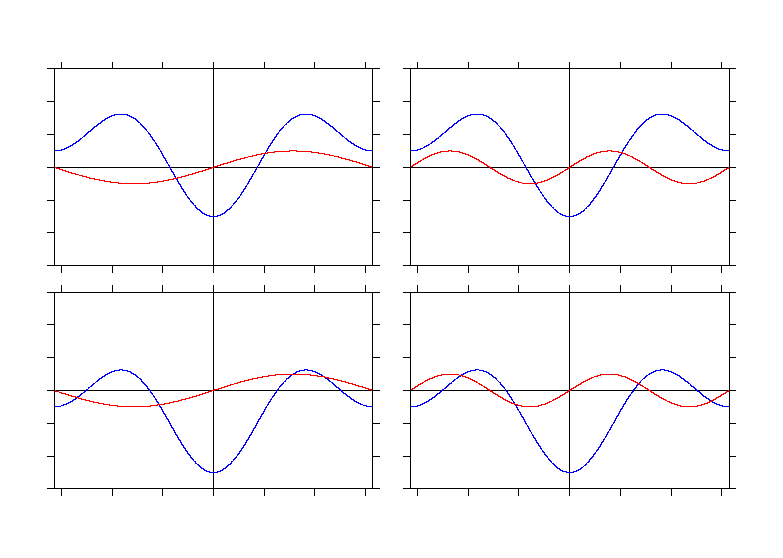
\includegraphics{Figures/Lattice.singlewire/dispersion/kdepend}}%
    \gplfronttext
  \end{picture}%
\endgroup

\caption{In blue: kinetic energy relative to chemical potential, $\varepsilon_k$. In red: pairing $\Delta_k$. Both in units of $t_1$ as a function of $kd$. Top row: $\mu = -0.5 t_1$. Bottom row: $\mu = 0.5 t_1$. Left column: $\Delta_k = \frac{t_1}{2}\sin(kd)$. Right column: $\Delta_k = \frac{t_1}{2}\sin(2kd)$. The bottom right figure is the only one, that exhibits $\nu = 2$, since we both need two zeroes for $k >0$ of $\varepsilon_k$ and a change in sign of $\Delta_k$ in-between these zeroes. For all figures we have set $t_2 = t_1$. }
\label{fig.dispersions.lattice}
\end{center}
\end{figure}

For the sake of clarity let us see, how we use this formula on the examples given in figure \ref{fig.dispersions.lattice}. Here we assume, that the pairing, shown in red, is either proportional to $\sin(kd)$ or $\sin(2kd)$, respectively the left and right column. The kinetic energy dispersion is shown in blue for two values of the chemical potential $\mu = -1/2$ and $\mu = 1/2$, top and bottom row respectively. The required \textit{two} zeroes of $\varepsilon_k$ for $\nu = 2$ is achieved in the bottom two figures. It is clear from the figure, that this is equivalent to a high filling fraction, since much of $\varepsilon_k$ must be negative. Further, we need the pairing to change sign in between the two zeroes of $\varepsilon_k$. Hence, a $\sin(2kd)$-like pairing is needed as well. This requirement means, that we need a high coherence length, because the $\sin(lkd)$ term of $\Delta_k$ is connected to pairing to the $l$'th neighbour. We will expand on this analysis in the following chapter, where we explicitly find the pairing using equation \eqref{eq.gapequation.lattice}.

